%================================================================================
% Erstellt am: 				14.07.2010
% Aufberarbeitet am:	06.09.2010
% Autor:							Thomas Karanatsios
%================================================================================

%Einbinden der Datei header.tex; diese enth�lt alle verwendeten Pakete,
%sowie �nderungen am Layout
%Da Latex f�r englischsprachige Texte ausgerichtet ist,
%wird als Dokumentenklasse das "`scrbook"' von Markus Kohm verwendet.
%Dieses ist f�r deutschsprachige Texte ausgelegt.
%BCOR12mm: 12mm Bindekorrektur (Verbreiterung des linken Randes)
%DIV11: entspricht in etwas der geforderten Textgr�sse und Seitenr�nder
%titlepage: eine Titelseite wird verwendet
%a4paper: DIN A4
%oneside: f�r eine sp�tere einseitige Bedruckung 
\documentclass[BCOR12mm,DIV11,titlepage,a4paper,oneside]{scrbook}

%Paket f�r deutsche Silbentrennung etc.
\usepackage{ngerman}
%\usepackage[latin1]{inputenc}

%Paket f�r Zeichenkodierung, entspricht UTF-8
%\usepackage[utf8x]{inputenc}
%(Tabellenfunktionen)
%\usepackage{booktabs}
%(Sonderschriftzeichen).
%\usepackage{pxfonts}

%Paket das die Ausgabefonts definiert
\usepackage[T1]{fontenc}

%Mathepakete
\usepackage{amsfonts}
\usepackage{amsmath}
\usepackage{cancel}
\usepackage{mathcomp}

\usepackage{pdfpages}

%\usepackage[options]{subfigure}

%Paket f�r das Einbinden von Grafiken �ber die figure-Umgebung
\usepackage{graphicx}
\usepackage{multirow}
\usepackage{array}


%Paket zum �ndern der Kopf- und Fusszeile
\usepackage{fancyhdr}
%Benutzt das Paket f�r eigenen Seitenstil
\pagestyle{fancy} 
%Erzeugt eine Linie in der Kopfzeile (l�sst sich mit 0.0pt ausblenden)
\renewcommand*{\headrulewidth}{0.4pt} 
\lhead{} %Kopfzeile links
\chead{} %Kopfzeile mitte
\rhead{\thepage} %Kopfzeile rechts
\lfoot{} %Fusszeile links
\cfoot{} %Fusszeile mitte
\rfoot{} %Fusszeile rechts
%�ndert die Seitennummerierung beim Inhaltsverzeichnis mit eigenem Stil
\renewcommand*{\indexpagestyle}{fancy}
%Verhindert die Seitennummerierung auf den Part-Seiten
\renewcommand*{\partpagestyle}{empty}
%�ndert die Seitennummerierung bei Chapter mit eigenem Stil
\renewcommand*{\chapterpagestyle}{fancy}


%Abbildungsnummerierung �ndern (abh�gig von chapter, z.B. Abbildung 1.1)
\renewcommand*{\thefigure}{\thechapter.\arabic{figure}}
%Tabellennummerierung �ndern (abh�ngig von chapter, z.B. Tabelle 1.1)
\renewcommand*{\thetable}{\thechapter.\arabic{table}}

%Paket zur pr�fix �nderung in Verzeichnissen

\usepackage[titles]{tocloft}

%Formatierung

%Paket, um ein Glossar/Abk�rzungsverzeichnis anzulegen
\usepackage{nomencl}
\let\abbrev\nomenclature
%Der Name wird in Glossar ge�ndert
\renewcommand{\nomname}{Abk�rzungsverzeichnis}
%Definiert die Aufteilung im Glossar zwischen Begriffen und Erl�uterung
\setlength{\nomlabelwidth}{.15\hsize}
%Definiert die Punktelinien im Glossar
%\renewcommand{\nomlabel}[1]{#1 \dotfill}
\setlength{\nomitemsep}{-\parsep}
%Veranlasst die Erstellung des Glossars
\makenomenclature

\setlength{\parindent}{0pt}

\usepackage{makeidx}
\makeindex

%Verhindern, dass eine neue Seite f�r ein einzelnes Wort/Zeile verwendet wird
\clubpenalty = 10000 % schliesst Schusterjungen aus 
\widowpenalty = 10000 % schliesst Hurenkinder aus (keine Beleidigung, sondern wirklich ein Fachbegriff)

%Paket f�r ein deutsches Literaturverzeichnis
%\usepackage{bibgerm}
%Paket f�r ein deutsches Literaturverzeichnis Contents lists
\usepackage[ngerman, english]{babel}

%Paket f�r die Verwendung von URLs durch den Befehl \url{}
\usepackage{url}

%Paket f�r Zeilenabstand (onehalfspace, singlespace)
\usepackage{setspace}

%Paket zur Erzeugung von Anf�hrungszeichen durch \enquote{Text}
\usepackage[ngerman]{babel}
\usepackage[babel, german=quotes]{csquotes}

%Paket f�r farbigen Text
%black,white,green,red,blue,yellow,cyan,magenta
\usepackage{color}

\usepackage{colortbl}

%Paket f�r farbigen Hintergrund f�r Verbatim-Umgebung (Quelltext-Umgebung)
\usepackage{fancyvrb}
\usepackage{verbatim,moreverb}
%Grauton f�r Quelltext-Umgebung definieren 80% Grau
\definecolor{sourcegray}{gray}{.80}
%Paket f�r Quelltext-Umgebung
\usepackage{listings}

%Paket f�r Positionierung der Objekte ohne Float (Verwendungsbsp.: \begin{figure}[H])
\usepackage{float}

%Paket zur Erzeugung von Hyperrefs und PDF Informationen
\usepackage[pdftex,plainpages=false,pdfpagelabels,
            pdftitle={Masterarbeit},
            pdfauthor={El Mehdi Bennani}
            ]{hyperref} 

%\usepackage[babel]{german}

\begin{document}

%=== Einleitung ======================================================
%Seitennummerierung Abstract bis einschliesslich Inhaltsverzeichnis
\frontmatter 
%Seitenzahlz�hler wird auf 3 gesetzt, da Titelseiten nicht mitgez�hlt werden
\setcounter{page}{3}
%Seitennummerierung findet in arabischen Zahlen statt 
\pagenumbering{arabic}
%Seitennummerierung in r�mischen Zahlen
%\pagenumbering{Roman}

%Einbinden der Titelseite
%!TEX root = ../montravail.tex

\begin{titlepage}

\begin{center}

%Logo der Fachhochschule K�ln
\begin{figure}[!ht]
	\centering
		
\includegraphics[natwidth=920pt, natheight=95pt, width=1.0\textwidth]{grafiken/logoheader.pdf}
\end{figure}

\vspace{0.8cm}

%Deutscher Titel
\begin{rmfamily}
%\textbf{\huge Transmover}\\
%\vspace{0.2cm}
\textbf{\huge DSL specification implementation TTCN3 \\ Domain Specific Language}\\
\normalsize
\end{rmfamily}
%
%\vspace{0.8cm}
%
%%Englischer Titel
%\begin{rmfamily}
%\textbf{Transmover}\\
%\large Development of a programmatic support exoskeleton robot \\and prototype implementation as a model\\
%\normalsize
%\end{rmfamily}

\vspace{1.2cm}

%Diplomarbeit 
%\begin{LARGE}
%\begin{scshape}
%\textbf{Diplomarbeit}\\[0.8em]
%\end{scshape}
%\end{LARGE}


\begin{LARGE}
\textbf{Master Thesis}\\
\end{LARGE}


\vspace{0.4cm}

%ausgearbeitet von...
\begin{large}
%Transmover\\
Author\\ 
\vspace{0.2cm}
\begin{LARGE}
\textbf{El Mehdi Bennani}\\
\end{LARGE}
\end{large}

%\vspace{0.6cm}
%
%%zur Erlangung des akademischen Grades...
%\begin{large}
%zur Erlangung des akademischen Grades\\
%\vspace{0.2cm}
%\textsc{Diplom Technischer Informatiker}\\
%\end{large}

\vspace{1.2cm}

%vorgelegt an der...
\begin{small}
vorgelegt an der\\ 
\vspace{0.4cm}
%\begin{scshape}
Fachhochschule K�ln\\
University of Applied Sciences Cologne\\
07 Fakult�t f�r Informations-, Medien- und\\
Elektrotechnik\\
%\end{scshape}
\end{small}

\vspace{1.2cm}

%im Studiengang...
\begin{small}
im Studiengang\\ 
\vspace{0.4cm}
%\textsc{
Technische Informatik \\
Matrikelnummer: 11033253 
\end{small}


\vspace{2.0cm}

%Autor der Masterarbeit und die Pr�fer
\begin{tabular}{rl}
        Erster Pr�fer:  &  Prof. Dr. Hans W. Nissen\\
       							    &  \small Fachhochschule K�ln \\[1.0em]
       Zweiter Pr�fer:  &  Professor Dr. Holger G�nther \\
       							    &  \small Fachhochschule K�ln \\
\end{tabular}

\vspace{0.6cm}

%Ort, Monat der Abgabe
\begin{large}
{\large \today}\\[4cm] % Date
%Koeln, September 2015
\end{large}

\end{center}

\newpage
\thispagestyle{empty}

%Kontaktm�glichkeiten des Autors und der Pr�fer
\begin{center}
\begin{tabular}{rl}
							&  \\[36.0em]
							
\large \textbf{Adressen:}	&  \quad El Mehdi Bennani\\
							&  \quad Mustermannstrasse 11\\
							&	 \quad 12345 Musterhausen\\
							&  \quad Muster@Muster.com\\[2.0em]
							
							&  \quad Professor Dr. Hartmut B�rwolff\\
							&  \quad Fachhochschule K�ln\\
							&  \quad Institut f�r Elektronik \\
							&  \quad und Informationsengineering\\
							&	 \quad Steinm�llerallee 1\\
							&	 \quad 51643 Gummersbach\\
							&  \quad Baerwolff@gm.fh-koeln.de\\[2.0em]
							
							&  \quad Professor Dr. Holger G�nther\\
							&  \quad Fachhochschule K�ln\\
							&  \quad Institut f�r Informatik\\
							&	 \quad Steinm�llerallee 1\\
							&  \quad 51643 Gummersbach\\
							&  \quad Guenther@gm.fh-koeln.de\\
\end{tabular}
\end{center}

\end{titlepage}

%Zeilenabstand 1,5 fach
%\onehalfspacing
%Einbinden des Abstracts bzw. der Kurzfassung
%!TEX root = ../montravail.tex

 
\chapter*{Abstract} 
\lhead[ \leftmark   ]{\textbf{Abstract}}
\addcontentsline{toc}{chapter}{\large{Abstract}}

Hier kommt die Kurzfassung hin


\chapter*{Abstract}

und das Abstract wenn ben�tigt

Anleitung:

Motivation des Textes: 
worin liegt die Bedeutung der entsprechenden Forschung, warum sollte der l�ngere Text gelesen werden?

%Somit erfolgt eine einfache Aufz�hlung
\begin{itemize}
	\item Fragestellung: welche Fragestellung(en) versucht der Text zu beantworten, was ist der
Umfang der Forschung, was sind die zentralen Argumente und Behauptungen?
	\item Methodologie: welche Methoden/Zug�nge nutzt der Autor/die Autorin, auf welche
empirische Basis st�tzt sich der Text?
	\item Methodologie: welche Methoden/Zug�nge nutzt der Autor/die Autorin, auf welche
empirische Basis st�tzt sich der Text?
	\item Ergebnisse: zu welchen Ergebnissen kam die Forschung, was sind die zentralen
Schlussfolgerungen des Textes?
	\item Implikationen: welche Schlussfolgerungen ergeben sich aus dem Text f�r die Forschung,
was f�gt der Text unserem Wissen �ber das Thema hinzu?
\end{itemize}



%Zeilenabstand f�r das Inhaltsverzeichnis 1 fach
%\singlespacing
%Einbinden des Inhaltsverzeichnis
%!TEX root = ../montravail.tex
\lhead[ \leftmark   ]{\textbf{Contents}}
\tableofcontents
%Zeilenabstand f�r den Hauptteil ist 1,5 fach
%\singlespacing
%!TEX root = ../montravail.tex

  %Erzeugt ein Abbildungsverzeichnis
	%F�gt die Zeile "Abbildungsverzeichnis" als Chapter ins Inhaltsverzeichnis ein
	\addcontentsline{toc}{chapter}{List of figures}
	\lhead[ \leftmark   ]{\textbf{List of figures}}
	%Erzeugt ein Abbildungsverzeichnis
	%Schreibt Abb.: vor die Abbildung
	\renewcommand{\cftfigpresnum}{Abb. }
	\renewcommand{\cftfigaftersnum}{:}
	\setlength{\cftfignumwidth}{2cm}
	\setlength{\cftfigindent}{0cm}
	\listoffigures
	%mit dieser Zeile wird das entsprechende Verzeichnis nach links geschrieben
	\lhead[ \leftmark   ]{\textbf{List of figures}}
	
	\newpage
	%F�gt die Zeile "Tabellenverzeichnis" als Chapter ins Inhaltsverzeichnis ein
	\addcontentsline{toc}{chapter}{List of tables}
	%Erzeugt ein Abk�rzungsverzeichnis	
	\newpage
	%Schreibt Tab.: vor die Abbildung
	\renewcommand{\cfttabpresnum}{Tab. }
	\renewcommand{\cfttabaftersnum}{:}
	\setlength{\cfttabnumwidth}{2cm}
	\setlength{\cfttabindent}{0cm}
	%mit dieser Zeile wird das entsprechende Verzeichnis nach links geschrieben
	\lhead[ \leftmark   ]{\textbf{List of tables}}	
	\listoftables
		
	\newpage
	%F�gt die Zeile "Glossar" als Chapter ins Inhaltsverzeichnis ein
	\addcontentsline{toc}{chapter}{List of abbreviations}
	\newpage
	%mit dieser Zeile wird das entsprechende Verzeichnis nach links geschrieben
	\lhead[ \leftmark   ]{\textbf{List of abbreviations}}
	\printnomenclature


%	\newpage
%	\chapter*{Vorwort}
%	\addcontentsline{toc}{chapter}{Vorwort}
%	\lhead[ \leftmark   ]{\textbf{Vorwort}}
%	
	\newpage
%die Aufgabenstellung l�sst sich auch als eigenes Kapitel schreiben/Speichern
	\chapter*{Topic}
	\addcontentsline{toc}{chapter}{Topic}
	%mit dieser Zeile wird das entsprechende Verzeichnis nach links geschrieben
	\lhead[ \leftmark   ]{\textbf{Topic}}
	
	Die Idee an einem Unterst�tzungs-Roboter f�r gehbehinderte Menschen zu forschen, entstand durch das medial wachsende
	Interesse an Laufrobotern. Diese sind bereits im Entertainmentbereich z. B. bei Spielzeugen g�ngig, werden aber inzwischen
	auch\\
	vermehrt f�r Milit�rzwecke eingesetzt....
%Zeilenabstand f�r den Hauptteil ist 1,5 fach
%\onehalfspacing

%=== Hauptteil =======================================================
%Seitennummerierung des Hauptteils
\mainmatter
%Nummerierung beginnt beim Hauptteil ab Seite 6 (muss angepasst werden)
\setcounter{page}{12}
	%Die Z�hler f�r Tabellen und Abbildungen werden zur�ckgesetzt, damit

%Einbinden eines Vorwortes
%!TEX root = ../Bachelorarbeit.tex

\chapter*{Vorwort}
\addcontentsline{toc}{chapter}{Vorwort}
\lhead[ \leftmark   ]{\textbf{Vorwort}}

Das Vorwort ist optional.

%Manchmal so wie hier Grau umrandet, ich hatte kein Vorwort folglich ist es bei mir auskommentiert
%\noindent{}\fcolorbox{black}{sourcegray}{\parbox{\textwidth}{
%	Diese Diplomarbeit entstand mit freundlicher Unterst�tzung der Fachhochschule K�ln
%	Campus Gummersbach, welche es erm�glichte Forschungen auf diesem Gebiet durchzuf�hren und somit das Projekt Transmover zu
%	zu initialisieren und vorzustellen. F�r das entgegengebrachte Vertrauen
%	und Unterst�tzung gilt mein Dank Herrn Professor Dr. Hartmut B�rwolff und
%	Herrn Professor Dr. Holger G�nther%}}
%	
%Abstand zwischen den Bl�cken
%	\vspace{0.75cm}
%	
%	%\noindent{}\fcolorbox{black}{sourcegray}{\parbox{\textwidth}{
%	Des weiteren m�chte ich meinen Eltern f�r Ihre Unterst�tzung im Studium
%	danken und Ihnen diese Arbeit widmen. F�r angeregte Diskussionen und fachliche Kommentare, gilt mein Dank auch meinen
%	Professoren und Kommilitonen der Fachhochschule K�ln Campus Gummersbach die diese Arbeit somit unterst�tzt haben.}}
	 	%in jedem Kapitel die Nummerierung neu beginnt
	
	\setcounter{chapter}{0}
	\setcounter{section}{1}
	\setcounter{table}{1}
	\setcounter{figure}{1}
	
	%Einbinden einer Einleitung
	\chapter*{Einleitung}
\addcontentsline{toc}{chapter}{Einleitung}
\lhead[ \leftmark   ]{\textbf{Einleitung}}
%!Das Vorwort ist optional.\\ \\

%Manchmal Grau umrandet dies macht man so ich hatte kein Vorwort folglich ist es bei mir auskommentiert
%\noindent{}\fcolorbox{black}{sourcegray}{\parbox{\textwidth}{
%Die Schicksale auf unserer Erde sind teilweise so verschieden und zahlreich, das es kaum m�glich sein wird den meisten Menschen Ihr Leben auf irgendeine Weise zu erleichtern oder sogar zu verbessern. 

%dies ist eine Mathematische Formel 
\begin{quotation}
\textit{\enquote{$A\rho\chi\eta\ \ \eta\mu\iota\sigma\upsilon\ \ \pi\alpha\nu\tau o \varsigma$ \\Der Anfang ist die H�lfte des Ganzen.}} (Vgl.\cite{111})
\end{quotation} 

%so wird eine korrekte Fu�note erstellt manche Professoren m�chten hier auch Lieteraturverweise sehen
Roboter\footnote{Der Begriff Roboter (tschechisch: robot) wurde von Josef und Karel Capek Anfang des 20. Jahrhunderts durch die Science-Fiction-Literatur gepr�gt. Der Ursprung liegt im slawischen Wort robota, welches mit Arbeit, Fronarbeit oder Zwangsarbeit �bersetzt werden kann. 1921 beschrieb Karel Capek in seinem Theaterst�ck R.U.R. in Tanks gez�chtete menschen�hnliche k�nstliche Arbeiter. Mit seinem Werk greift Capek das klassische Motiv des Golems auf. Heute w�rde man Capeks Kunstgesch�pfe als Androiden bezeichnen. Vor der Pr�gung dieses Begriffes wurden Roboter zum Beispiel in den Werken von Stanislaw Lem als Automaten oder Halbautomaten bezeichnet.}

%� wird in dieser Arbeit wie folgt gemacht
Bei R�dern und Ketten ist dies hingegen nicht der Fall, Sie brauchen gro\ss fl�chige St�tzpunkte. 

%Zitate werden genormt so gemacht
Das bedeutet, dass letztere Arten der Fortbewegung einen ununterbrochenen Kontakt zum Boden ben�tigen. (Vgl.\cite{116})\\
%Allerdings fehlt hier noch die Seitenangabe "{Seite 4, ff}" das verlangen nicht alle Professoren so wie meiner 

%f�r den Index verwendete W�rter werden so angegeben
Dadurch wurden die im Verlauf der Evolution optimierten Konstruktionen von Beinen, das Zusammenspiel von Sensorik\index{Sensorik} und Aktorik\index{Aktorik} und die Steuerung von Gehbewegungen weitestgehend analysiert und dienten somit dem besseren Verst�ndnis der Laufmotorik\footnote{Die Laufmotorik beinhaltet die Bewegungsfunktion und deren Lehre, die F�higkeit des K�rpers sich kontrolliert zu bewegen, die Gesamtheit der vom zentralen Nervensystem kontrollierten Bewegungen des K�rpers im Gegensatz zu den unwillk�rlichen Reflexen des K�rpers und die Unterscheidung in Grob- und Feinmotorik}\index{Laufmotorik}.\\\\ 

An dieser Stelle sei darauf hingewiesen, dass dieses Forschungsgebiet einen stark interdisziplin�ren Charakter besitzt...


%Falls eine neue Seite erzwungen werden soll macht man dies so
\newpage
%um den Text Fett zu schreiben wir dieser Befehl verwendet
\textbf{Kapitel�bersicht}\\\\  	%in jedem Kapitel die Nummerierung neu beginnt
	
	\setcounter{chapter}{0}
	\setcounter{section}{1}
	\setcounter{table}{1}
	\setcounter{figure}{1}
	
%Einbinden des ersten Kapitels
%!TEX root = ../Bachelorarbeit.tex

\chapter{Grundlagen}
%\addcontentsline{toc}{chapter}{Grundlagen}
\lhead[ \leftmark   ]{\textbf{Grundlagen}}

%erstes Unterkapitel
\section{Erste �berschrift}

Hier schreiben
%n�chstes unterkapitel ebene 2
\subsection{Zweite �berschrift}
Hier schreiben

%unterkapitel Ebene 3 nicht im Inhaltsverzeichnis aufgef�hrt! 
\subsubsection{Dritte �berschrift}
\textit{hier kann Kursiv geschrieben werden}

%zweites Unterkapitel
\section{Erste �berschrift}

%n�chstes unterkapitel ebene 2
\subsection{Zweite �berschrift}

%Abbildungsbeispiel
%Abbildungsquelle immer! angeben es sei den selber gemacht!!!!
Text....(siehe Abb. 1.1)

\begin{figure}[!ht]
	%mitte der Seite
	\centering
		%[nat�rliche Breite in Pixeln, nat�rliche H�he in Pixeln, Abh�ngigkeit von der Textbreite]
		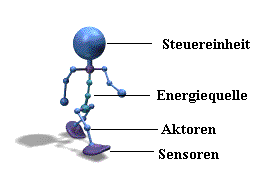
\includegraphics[natwidth=1200pt, natheight=349pt, width=0.4\textwidth]{grafiken/Robotpeintre.PNG}
	\caption[Aufbau allgemein]{Aufbau und Komponenten von Robotern}
	\label{fig:Aufbau und Komponenten von Robotern}
\end{figure}

%unterkapitel Ebene 3 nicht im Inhaltsverzeichnis aufgef�hrt!
\subsubsection{Dritte �berschrift}

%Aufz�hlung
\begin{itemize}
	\item Die Bewegungsform der Achsen
	\item Anzahl und Anordnung der Achsen
	\item Die Formen des Arbeitsraums
\end{itemize}
    
... Arm zu strecken. (Vgl.\cite{112}) 
%n�chstes unterkapitel ebene 2
\subsection{Zweite �berschrift}
%unterkapitel Ebene 3 nicht im Inhaltsverzeichnis aufgef�hrt!
\subsubsection{Dritte �berschrift}
Hier Text einf�gen\index{einf�gen}

%� ohne weiterf�hrung des Wortes
Roboterfu\ss \ befindet

homogene\\ 4 x 4  Matrix:

\begin{equation} 
T = \begin{pmatrix}
     Ax&Ay&Az&0\\Bx&By&Bz&0\\Cx&Cy&Cz&0\\Px&Py&Pz&1
     \end{pmatrix}
\end{equation}


\begin{equation}(\theta, d, a, \alpha)\end{equation}
 
verschiedene Matrizen:

\begin{equation}
T=\begin{pmatrix}\cos\theta & -\sin\theta \cos\alpha & \sin\theta \sin\alpha & \arccos\theta\\ \sin\theta & \cos\theta \cos\alpha & -\cos\theta \sin\alpha & \arcsin\theta\\ 0 & \sin\alpha & \cos\alpha & d\\ 0 & 0 & 0 & 1\end{pmatrix}
\end{equation}

\begin{equation}
^{n - 1}T_n
  = \begin{pmatrix}
    \cos\theta_n & -\sin\theta_n \cos\alpha_n & \sin\theta_n \sin\alpha_n & a_n \cos\theta_n \\
    \sin\theta_n & \cos\theta_n \cos\alpha_n & -\cos\theta_n \sin\alpha_n & a_n \sin\theta_n \\
    0 & \sin\alpha_n & \cos\alpha_n & d_n \\
    0 & 0 & 0 & 1
  \end{pmatrix}.
\end{equation}


\begin{equation}
T=T_1T_2T_3T_4T_5T_{tcp}
\end{equation}


%Beispiel f�r eine Tabelle
Text...(Siehe Tab. 1.1)
\\\\
\textbf{Titel:}\\%Der Titel bei Tabellen muss immer �ber der Tabelle stehen Statuten FH-Koeln! bei Abbildungen drunter! 
\begin{table}[ht]
\centering
\caption[Titel]{Titel}	
	 \begin{tabular}{|c|p{11cm}|}
			\hline
			\rowcolor{sourcegray}
			\textbf{�berschrift 1} & \textbf{�berschrift 2}\\
			\hline
			Text & Text \newline 
						 Text\\
			\hline
			Text & Text \newline 
						 Text\\
			\hline
		\end{tabular}
	\vspace{1.0em}
	%\caption[Mobilit�tsgrade]{Gliederung der Mobilit�tsgrade}
	\label{tab:Titel}
\end{table}

\newpage
%Beispiel f�r zwei Bilder nebeneinander
\begin{figure}[!ht]
\centering 
\begin{minipage}[hbt]{7cm}
	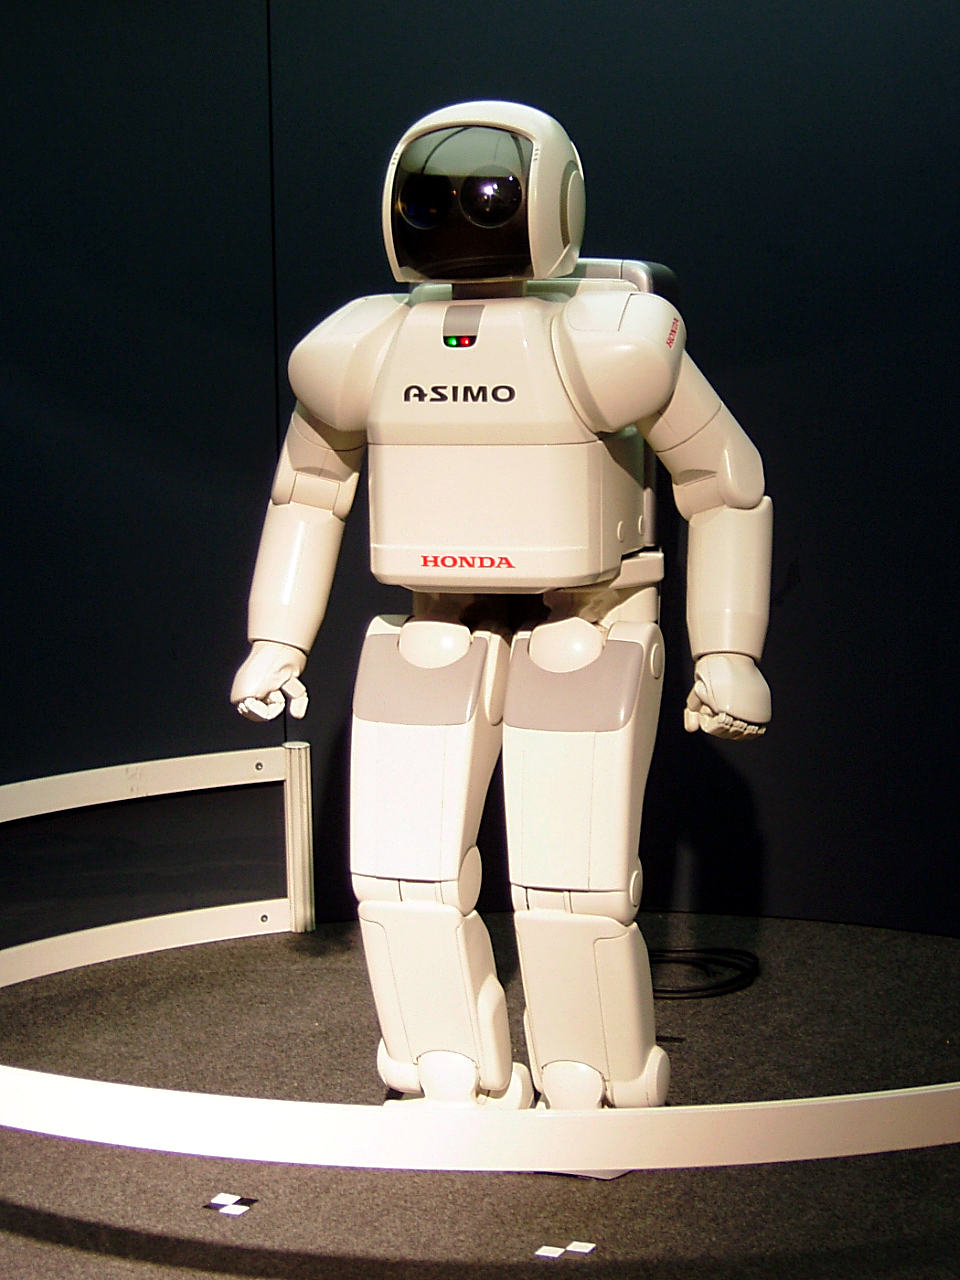
\includegraphics[width=7cm]{grafiken/HONDA_ASIMO.jpg}
\end{minipage}
\begin{minipage}[hbt]{6.7cm}
	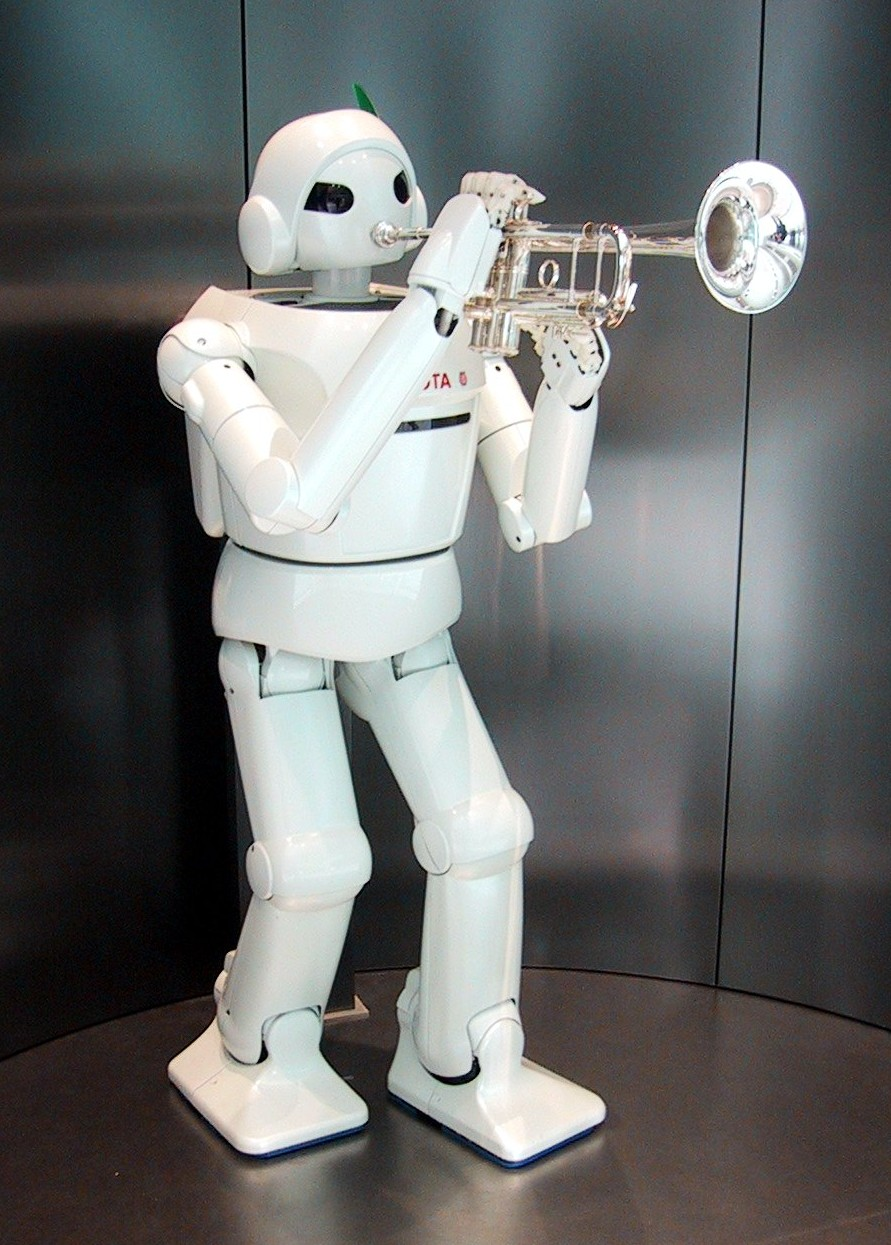
\includegraphics[width=6.7cm]{grafiken/Toyota_Robot_at_Toyota_Kaikan.jpg}
	\end{minipage}
	\caption[Humanoide Roboter]{Humanoide Roboter Links der Aibo von Honda rechts der Roboter von Toyota}
	\label{Humanoide Roboter}
\end{figure}

Bild-Quellen:(\url{http://de.wikipedia.org/wiki/Humanoider_Roboter})\\Sichtung: 17.09.2010\\\\

In Abb. 1.2 sind...Text\\\\
 
%�bersichtshalber besser Begriffe betonen
Kraft \textbf{F}, der Masse \textbf{m} und der Beschleunigung \textbf{a} kann mit der daraus resultieren Formel die Kraft, die wirkt, berechnet werden: \begin{equation}F = m * a \end{equation} Folglich ist die Kraft das Produkt von Masse und Beschleunigung.  

%Formeln 
SI-Einheit der Kraft:
\begin{equation}
[F] = kg * \frac{m}{s^{2}} = Newton (N)
\end{equation}

\begin{equation}M = F * l = F * r * \sin\alpha \end{equation}
 
SI-Einheit des Drehmomentes: \begin{equation}[M] = Newtonmeter (N * m)\end{equation}
  

	%Die Z�hler f�r Tabellen und Abbildungen werden zur�ckgesetzt, damit
	%in jedem Kapitel die Nummerierung neu beginnt
	\setcounter{table}{1}
	\setcounter{figure}{1}
 %Einbinden des ersten Kapitels
%!TEX root = ../Bachelorarbeit.tex

\chapter{Marktanalyse}
\lhead[ \leftmark   ]{\textbf{Marktanalyse}}
Aufbau siehe Kapitel 1

%Aufbau des Abk�rzungsverezeichnisses muss nicht hier stehen geht in jedem Kapitel
%======================================================================
%======================================================================
%Eintrag ins Abk�rzungsverzeichnis
\nomenclature{IBK}{Initialer Bodenkontakt}
\nomenclature{BA}{Belastungsantwort}
\nomenclature{BIC}{Business Innovation Center}
\nomenclature{USB}{Universal Serial Bus}
\nomenclature{KOS}{Koordinatensysteme}
\nomenclature{TCP}{Tool Center Point}
\nomenclature{SIG}{Special Interest Group}
\nomenclature{WPAN}{Wireless Personal Area Network}
\nomenclature{SRD}{Short Range Devices}
\nomenclature{ISM-Band}{Industrial, Scientific and Medical Band}
\nomenclature{WLAN}{Wireless Local Area Network}
\nomenclature{EDR}{Enhanced Data Rate}
\nomenclature{SPP}{Serial Port Profile}
\nomenclature{LAN}{Local Area Network}
\nomenclature{MKS}{Mehrk�rpersystem}
\nomenclature{DFG}{Deutsche Forschungsgemeinschaft}
\nomenclature{JARA}{Japan Robot Association}
\nomenclature{RIA}{Robot Institut of America}
\nomenclature{VDI}{Verein Deutscher Ingenieure}
\nomenclature{ISO}{International Organization for Standardization}
\nomenclature{IEEE}{Institute of Electrical and Electronics Engineers}
\nomenclature{MPL}{Mozilla Public License}
\nomenclature{Pose}{Position und Orientierung}
\nomenclature{SOC}{System on a Chip}
\nomenclature{CAN}{Controller Area Network}
\nomenclature{LIN}{Local Interconnect Network}
\nomenclature{MCU}{Mikrocontroller Unit}
\nomenclature{ISC}{Inter-Integrated Circuit}
\nomenclature{SPI}{Serial Peripheral Interface}
\nomenclature{LCD}{Liquid Crystal Display}
\nomenclature{PWM}{Pulse Width Modulation}
\nomenclature{ROM}{Read only Memory}
\nomenclature{EPROM}{Erasable Programmable Read Only Memory}
\nomenclature{UV}{Ultra Violet}
\nomenclature{OTP}{One Time Programmable}
\nomenclature{RAM}{Random Acess Memory}
\nomenclature{ARM7}{Advanced RISC Machines}
\nomenclature{PDA}{Personal Digital Assistant}
\nomenclature{CSR}{Core Serial Protocol}
\nomenclature{OS}{Oberschenkel}
\nomenclature{MSw}{Mittlere Schwungphase}
\nomenclature{TD}{Touch Down}
\nomenclature{MSt}{Mittlere Standphase}
\nomenclature{TSt}{Terminale Standphase}
\nomenclature{VSw}{Vor-Schwungphase}
\nomenclature{TSw}{Terminale Schwungphase}
\nomenclature{TO}{Take Off}
\nomenclature{ISw}{Initiale Schwungphase}
\nomenclature{SG}{Sprunggelenk}
\nomenclature{KG}{Kniegelenk}
\nomenclature{KI}{K�nstliche Intelligenz}
\nomenclature{DOF}{Degrees of freedom}




\newpage
%\addcontentsline{toc}{chapter}{Ergebnisse}
\lhead[ \leftmark   ]{\textbf{Ergebnisse}}
\section{dfhdhgj}
Aufbau siehe Kapitel 1 

\section{thsgfnfgnj}
Text

\section{gfhfgjdrtu}
Text

	
	%Die Z�hler f�r Tabellen und Abbildungen werden zur�ckgesetzt, damit
	%in jedem Kapitel die Nummerierung neu beginnt
	\setcounter{table}{1}
	\setcounter{figure}{1}
	%Einbinden des zweiten Kapitels
%!TEX root = ../Montravail.tex

\chapter{Entwicklung des Modells}
\lhead[ \leftmark   ]{\textbf{Modell Realisierung}}
Aufbau siehe Kapitel 1 

\section{Erstes Unterkapitel}
%Beispiel f�r nummerierte Aufz�hlung
\begin{enumerate}
	\item Text\\
	Text
	\item Text\\
	Text
	\item Text\\
	Text
\end{enumerate} 

\newpage
%Eingaben von Source Code
Zuerst erfolgt zum besseren Verst�ndnis die Deklarierung der verwendeten Variablen\\
\begin{lstlisting}[basicstyle=\small,numbers=left,numberstyle=\footnotesize\small,backgroundcolor=\color{sourcegray}]
// die Motoren des rechten Beines werden wie in dem bisher 
// verwendeten Schema zugewiesen 
// H�fte (C), Knie (B) und Fussgelenk (A)
public static Motor motorHip = new Motor(MotorPort.C);
public static Motor motorKnee = new Motor(MotorPort.B);
public static Motor motorAnkle = new Motor(MotorPort.A);
public static boolean sensorReached1 = false;

// der Ultraschallsensor wird an Port S1 erwartet
public static UltrasonicSensor sonicSensor1 = 
              new UltrasonicSensor(SensorPort.S1);

//Der TouchSensor wird an Port S2 erwartet und wird zum iterieren
// durch einen Bewegungsablauf verwendet
public static TouchSensor touchSensor = 
              new TouchSensor(SensorPort.S2);
	
\end{lstlisting}

%\noindent{}Beispiel f�r eine nummerierte Aufz�hlung:
\begin{enumerate}
	\item Item 1
	\item Item 2	
	\item Item 3
\end{enumerate}

%\noindent{}Beispiel f�r eine unnummerierte Aufz�hlung mit neuem Symbol:
\begin{itemize}
\renewcommand{\labelitemi}{$\rightarrow$}
	\item Item 1
	\item Item 2
	\item Item 3
\end{itemize}

%Referenz zu Grafik \ref{fig:showcase} in Kapitel \ref{sec:section}.


	
	%Die Z�hler f�r Tabellen und Abbildungen werden zur�ckgesetzt, damit
	%in jedem Kapitel die Nummerierung neu beginnt
	\setcounter{table}{1}
	\setcounter{figure}{1}
	%Einbinden des zweiten Kapitels
%!TEX root = ../Bachelorarbeit.tex

\chapter{Ergebnisse}
%\addcontentsline{toc}{chapter}{Ergebnisse}
\lhead[ \leftmark   ]{\textbf{Ergebnisse}}
\section{Pr�sentation}
Aufbau siehe Kapitel 1 

\section{Schwierigkeiten}
Text

\section{Auswertungen}
Text

	%Die Z�hler f�r Tabellen und Abbildungen werden zur�ckgesetzt, damit
	%in jedem Kapitel die Nummerierung neu beginnt
	\setcounter{table}{1}
	\setcounter{figure}{1}
	%Einbinden des zweiten Kapbitels

\chapter{Zusammenfassung}
%\addcontentsline{toc}{chapter}{Zusammenfassung und Ausblick}
\lhead[ \leftmark   ]{\textbf{Zusammenfassung und Ausblick}}
\section {Zusammenfassung}
Text

\section{Ausblick auf zuk�nftige Arbeiten}
Text

\section{Schlusswort}
Text

%Zeilenabstand 1 fach f�r die Verzeichnisse
%\halfspacing
\singlespacing
%Einbindne der Verzeichnisse
%!TEX root = ../montravail.tex
  
  %Erzeugt ein Abbildungsverzeichnis
%	\listoffigures
	%F�gt die Zeile "`Abbildungsverzeichnis"' als Chapter ins Inhaltsverzeichnis ein
%	\addcontentsline{toc}{chapter}{Abbildungsverzeichnis}
	
	%Erzeugt ein Tabellenverzeichnis
%	\listoftables
	%F�gt die Zeile "`Tabellenverzeichnis"' als Chapter ins Inhaltsverzeichnis ein
%	\addcontentsline{toc}{chapter}{Tabellenverzeichnis}
	
	%Erzeugt ein Glossar
%	\printnomenclature
	%F�gt die Zeile "`Glossar"' als Chapter ins Inhaltsverzeichnis ein
%	\addcontentsline{toc}{chapter}{Glossar}

	%Erzeugt ein Glossar
%	\printnomenclature
	%F�gt die Zeile "Glossar" als Chapter ins Inhaltsverzeichnis ein
%	\addcontentsline{toc}{chapter}{Glossar}
	
			
%	%�ndert den Stil des Literaturverzeichnisses
%  \bibliographystyle{geralpha}
%	%Erzeugt das Literaturverzeichnis anhand der Datei "`literatur.bib"'
%	\bibliography{literatur}
%	%F�gt die Zeile "`Literaturverzeichnis"' als Chapter ins Inhaltsverzeichnis ein
%	\addcontentsline{toc}{chapter}{Literaturverzeichnis}
	
	

%=== Schlussteil =====================================================
%%Seitennummerierung f�r den Anhang
%\backmatter
%Seitennummerierung in r�mischen Zahlen
%\pagenumbering{Roman}

	%�ndert den Stil des Literaturverzeichnisses
  \lhead[ \leftmark   ]{\textbf{Literaturverzeichnis}}
  \bibliographystyle{geralpha}
	%Erzeugt das Literaturverzeichnis anhand der Datei "`literatur.bib"'
	\bibliography{literatur}
	%F�gt die Zeile "`Literaturverzeichnis"' als Chapter ins Inhaltsverzeichnis ein
	\addcontentsline{toc}{chapter}{\large{Literaturverzeichnis}}

	
%F�gt die Zeile "`Anhang"' als Part ins Inhaltsverzeichnis (toc = table of content) ein
%\addcontentsline{toc}{chapter}{Anhang}
%Einbinden des Anhangs mit s�mtlichen Verzeichnissen
%\singlespacing

%!TEX root = ../Bachelorarbeit.tex

\part*{Anhang}
\addcontentsline{toc}{part}{Anhang}
\lhead[ \leftmark   ]{\textbf{Anhang}}
%\addcontentsline{toc}{chapter}{Anhang}

\chapter*{Inhalt Anhang}

\textbf{Auf der mitgelieferten CD befindliche Dateien:}\\
\begin{enumerate}
	\item Video der Ergebnisse des entwickelten Transmovers 
	\item Marktanalyse
		\begin{itemize}
			\item BIC Analyse
			\item Frageb�gen befragter Betroffener
		\end{itemize}
	\item Skizzen und Entw�rfe
		\begin{itemize}
			\item Skizze
			\item Entwurf LEGO Designer
		\end{itemize}
	\item Programmablaufpl�ne
	\item Excel Datei Auswertung Winkelmessung
	\item Sequenzdiagramme
	\item Quellcodes
		\begin{itemize}
			\item Winkeleinmessung
			\item Transmover LabVIEW Programme
			\item Transmover JAVA Programme
			\item Wii Remote Programme
		\end{itemize}
\end{enumerate}

%Zeilenabstand 1 fach f�r den Eid

%\singlespacing
%Einbinden des Eides
%!TEX root = ../Bachelorarbeit.tex

\chapter*{Erkl�rung}
\addcontentsline{toc}{part}{Erkl�rung}
\lhead[ \leftmark   ]{\textbf{Erkl�rung}}
Ich versichere, die von mir vorgelegte Arbeit selbst�ndig verfasst zu haben.\\ \\
Alle Stellen, die w�rtlich oder sinngem�\ss \ aus ver�ffentlichten Arbeiten anderer entnommen sind, habe ich als entnommen kenntlich gemacht. S�mtliche Quellen und Hilfsmittel, die ich f�r die Arbeit benutzt habe, sind angegeben.\\ \\
Die Arbeit hat nach meinem Wissen mit gleichem Inhalt noch keiner anderen Pr�fungsbeh�rde vorgelegen.
\vspace{1.5cm}
\\
Gummersbach, 14. Oktober 2010
\vspace{2cm}
\\
Thomas Karanatsios


%F�gt die Zeile "`Glossar"' als Chapter ins Inhaltsverzeichnis ein
%\addcontentsline{toc}{chapter}{Glossar}
%Zeilenabstand 1 fach f�r die Verzeichnisse
%\singlespacing
%Einbindne der Verzeichnisse
%\singlespacing
%Das Glossar ist Optional und mit Tabellen etwas getrickst 
%es geht bestimmt auch anders aber ich hatte leider keine Zeit mehr bei meiner Arbeit das zu machen.
\chapter*{Glossar}
\addcontentsline{toc}{part}{Glossar}
\lhead[ \leftmark   ]{\textbf{Glossar}}
\begin{table}[!ht]	
	 \begin{tabular}{ l p{10cm}}
			\textbf{Autonom} 			& das Programm welches implementiert ist arbeitet weitgehend unabh�ngig von Benutzer eingriffen. \tabularnewline [7pt]
			\textbf{Biometrie} 		& Die Biometrie auch Biometrik genannt besch�ftigt sich mit Messungen an Lebewesen und den dazu erforderlichen Mess- und Auswerteverfahren.\tabularnewline [7pt]
			\textbf{Bionisch} 		& Adjektiv zur Beschreibung eines Organismus, dessen biologische Grundlage durch technische
															M�glichkeiten verbessert wurde.\tabularnewline [7pt]
			\textbf{Degrees of freedom} & (DOF) bedeutung Freiheitsgrade = Der Freiheitsgrad bezeichnet einen Parameter eines Systems. Die Eigenschaft, ein Freiheitsgrad zu sein, ergibt sich f�r einen Parameter
																		daraus, Mitglied in einer Menge von Parametern zu sein, die das System beschreiben.\tabularnewline [7pt]
			\textbf{Deliberativ} 	& Deliberativ = erw�gen, �berlegen, sich
															entscheiden, beschlie\ss en ist eine semantische Funktion Verbmodus des Konjunktivs z. B. im
															Lateinischen (coniunctivus deliberativus), die eine �berlegende R�ckfrage als Reaktion auf eine
															Aufforderung ausdr�ckt.\tabularnewline [7pt]
			\textbf{Dynamik} 				& Eine Dynamik steht f�r, das Teilgebiet der Mechanik, das sich mit der Wirkung von Kr�ften befasst\tabularnewline [7pt]												
			\textbf{Endeffektor} 	& Als Endeffektor wird in der Robotik das letzte Element einer kinematischen Kette bezeichnet. Bei 
															Industrierobotern kann es sich hierbei zum Beispiel um eine Einheit zum Schwei\ss en von
															Autokarosserien oder allgemein um einen einfachen Greifer handeln. Der im englischen als TCP
															(Tool Center Point) bezeichnete ausgezeichnete Punkt am Ende der kinematischen Kette ist das
															Zielsystem, f�r das die aus der gestellten Aufgabe resultierenden Positionierunganforderungen
															gelten. Aufgaben spezifisch kann der TCP dabei auch au\ss erhalb des Roboters liegen, Beispiele
															w�ren der Fokus eines gegriffenen Lasers oder auch die Mitte des gerade transportierten
															Objekts.\tabularnewline [7pt]									
%			\textbf{Exoskelett} 	& Ein Exoskelett ist eine St�tzstruktur f�r einen Organismus, das eine stabile �u\ss ere H�lle um diesen bildet.\tabularnewline [7pt]							
		\end{tabular}
	\vspace{1.0em}
\end{table}


\newpage
\begin{table}[!ht]	
	 \begin{tabular}{ l p{10cm}}
	 		\textbf{Dorsalextension} 	& steht f�r die Bewegung in den Zehengelenken in Richtung Fu\ss r�cken.\tabularnewline [7pt]				
	 		\textbf{Extension} 		& Die Extension (von lat. extensio "Streckung") ist die Streckung eines Gelenkes. Die gegenl�ufige
															Bewegung wird als Flexion bezeichnet.\tabularnewline [7pt]																
			\textbf{Exoskelett} 	& Ein Exoskelett ist eine St�tzstruktur f�r einen Organismus, das eine stabile �u\ss ere H�lle um diesen bildet.\tabularnewline [7pt]					
	 	 	\textbf{Energy Harversting} & Als Energy Harvesting (w�rtlich �bersetzt Energie-Ernten) bezeichnet man die Erzeugung von
																		Strom aus Quellen wie Umgebungstemperatur, Vibrationen oder Luftstr�mungen. Die Industrie
																		entwickelt bereits heute Energiequellen f�r drahtlose Sensornetzwerke oder Anwendungen wie
																		etwa Fernbedienungen an schwer erreichbaren Stellen. Energy Harvesting vermeidet bei
																		Drahtlostechnologien Einschr�nkungen durch kabelgebundene Stromversorgung oder
																		Batterien.\tabularnewline [7pt]			
	 		\textbf{Flexion} 						& Die gegenl�ufige Bewegung zur Extension wird als Flexion bezeichnet.\tabularnewline [7pt]
			\textbf{Inertialsystem} 		& In der Physik ist ein Inertialsystem (von lat. iners "unt�tig, tr�ge") ein Koordinatensystem, in dem sich kr�ftefreie K�rper geradlinig, gleichf�rmig bewegen. In
																		einem Inertialsystem gilt also das newtonsche Tr�gheitsgesetz in seiner einfachsten Form, nach der kr�ftefreie K�rper ihre Geschwindigkeit in Betrag und Richtung
																		beibehalten und Beschleunigungen proportional zur anliegenden Kraft erfolgen. Der Begriff Inertialsystem wurde erstmals von Ludwig Lange (1885) verwendet.\tabularnewline
																		[7pt]
			\textbf{Inhibition} 				& Das Wort Inhibition (lat. inhibere "unterbinden", "anhalten"; veraltend Inhibierung, deutsch Hemmung, Antonym Desinhibition, Desinhibierung) bezeichnet:
																		in der Neurobiologie eine Abnahme der Erregbarkeit von Nervenzellen, siehe Inhibition (Neuron)
																		in der Ethologie die Blockierung einer Verhaltensweise durch innere oder �u\ss ere Faktoren, siehe Bedingte Hemmung
																		in der Digitaltechnik bezeichnet die Inhibition eine Schaltung aus einem UND- und einem NICHT-Glied, siehe Inhibition (Digitaltechnik)\tabularnewline [7pt]
			\textbf{Ipsilateral} 				& Ipsilateral bedeutet "auf derselben K�rperseite oder -h�lfte gelegen".
																		Das Gegenteil von ipsilateral ist kontralateral. \tabularnewline [7pt]
		\end{tabular}
	\vspace{1.0em}
\end{table}

\newpage
%\addcontentsline{toc}{part}{Index}
%\chapter*{Index}
\addcontentsline{toc}{part}{Index}
\lhead[ \leftmark   ]{\textbf{Index}}
\printindex

\newpage
\lhead[ \leftmark   ]{\textbf{Widmung}}
\textbf{\LARGE Widmung}\\\\
Die Widmung ist optional!
Text\\\\

In Liebe,\\ 
Euer Sohn

\end{document}